\documentclass[10pt]{beamer}

\usepackage[utf8]{inputenc}
\usepackage[english,russian]{babel}

\usetheme{metropolis}
\usepackage{appendixnumberbeamer}

\usepackage{booktabs}
\usepackage[scale=2]{ccicons}

\usepackage{pgfplots}
\usepgfplotslibrary{dateplot}

\usepackage{xspace}
\newcommand{\themename}{\textbf{\textsc{metropolis}}\xspace}

\usepackage{cite,enumerate,float,indentfirst}
\usepackage{tcolorbox}
\usepackage{alltt}
\usepackage{multicol}
\usepackage{listings}

\graphicspath{{images/}}

\newcommand{\itemi}{\item[\checkmark]}

\title{Ассамблея}
\subtitle{Мультиязычный обфускатор программ и компилируемая библиотека непрозрачных предикатов}
\date{\today}
\author{Антон Баглий, Борис Штейнберг, Елена Алымова, Константин Гуфан}
\institute{ЮФУ, ФГАНУ Спецвузавтоматика}
% \titlegraphic{\hfill
\includegraphics[height=1.5cm]{logo.pdf}}



\begin{document}


\begingroup
\setbeamertemplate{footline}{\vspace*{-1cm}\centering Языки программирования и компиляторы 2017\par} 
\begin{frame}
  \titlepage
\end{frame}
\endgroup


\begin{frame}
\frametitle{Первоначальные цели и ограничения}
\begin{itemize}
  \item \textbf{Предназначение:} Пооператорное запутывание байт-кода MSIL, LLVM и исходного текста JavaScript
  \item \textbf{Функции:} 
  \begin{itemize}
    \item Описание преобразований операторов общее для всех входных языков 
    \item Поиск подходящих операторов и применение преобразований к ним
    \item Вставка вызовов или inlining непрозрачных функций, указанных в описании преобразований
  \end{itemize}
  \item \textbf{Ограничения:} 
  \begin{itemize}
    \item Обработка каждой инструкции (оператора) отдельно
    \item Одно представление для всех входных языков
  \end{itemize}
\end{itemize}
\end{frame}

\begin{frame}
\frametitle{Сложности}

\begin{columns}
 
\column{0.4\textwidth}
\begin{itemize}
\item Сложно создать новое универсальное представление для очень разных входных языков
\item Структура исходной программы должна представляться одинаково для всех языков
\end{itemize}
 
\column{0.6\textwidth}
\begin{tcolorbox}[colback=green!5,colframe=green!40!black,title=решения]
\begin{itemize}
\item Используется готовое AST с аннотациями произвольного типа, в которые помещаются части исходной программы
и другая информация (например, типы)
\item Структура графа потока управления с вершинами-простыми блоками подходит больше всего
\end{itemize}
\end{tcolorbox}
\end{columns}

\end{frame}

\begin{frame}
\frametitle{Реализованные средства и алгоритмы}
\begin{itemize}
  \item Описание преобразований - InterCode
  \item Применение преобразований к арифметическим операторам в MSIL, LLVM, JavaScript
  \item Проверка типов при применении преобразований в MSIL и LLVM
  \item Вставка непрозрачных функций, если они указаны в преобразовании
  \item Библиотека непрозрачных функций
\end{itemize}
\end{frame}

\begin{frame}
\frametitle{Модули}
\begin{figure}[H]
  \center
  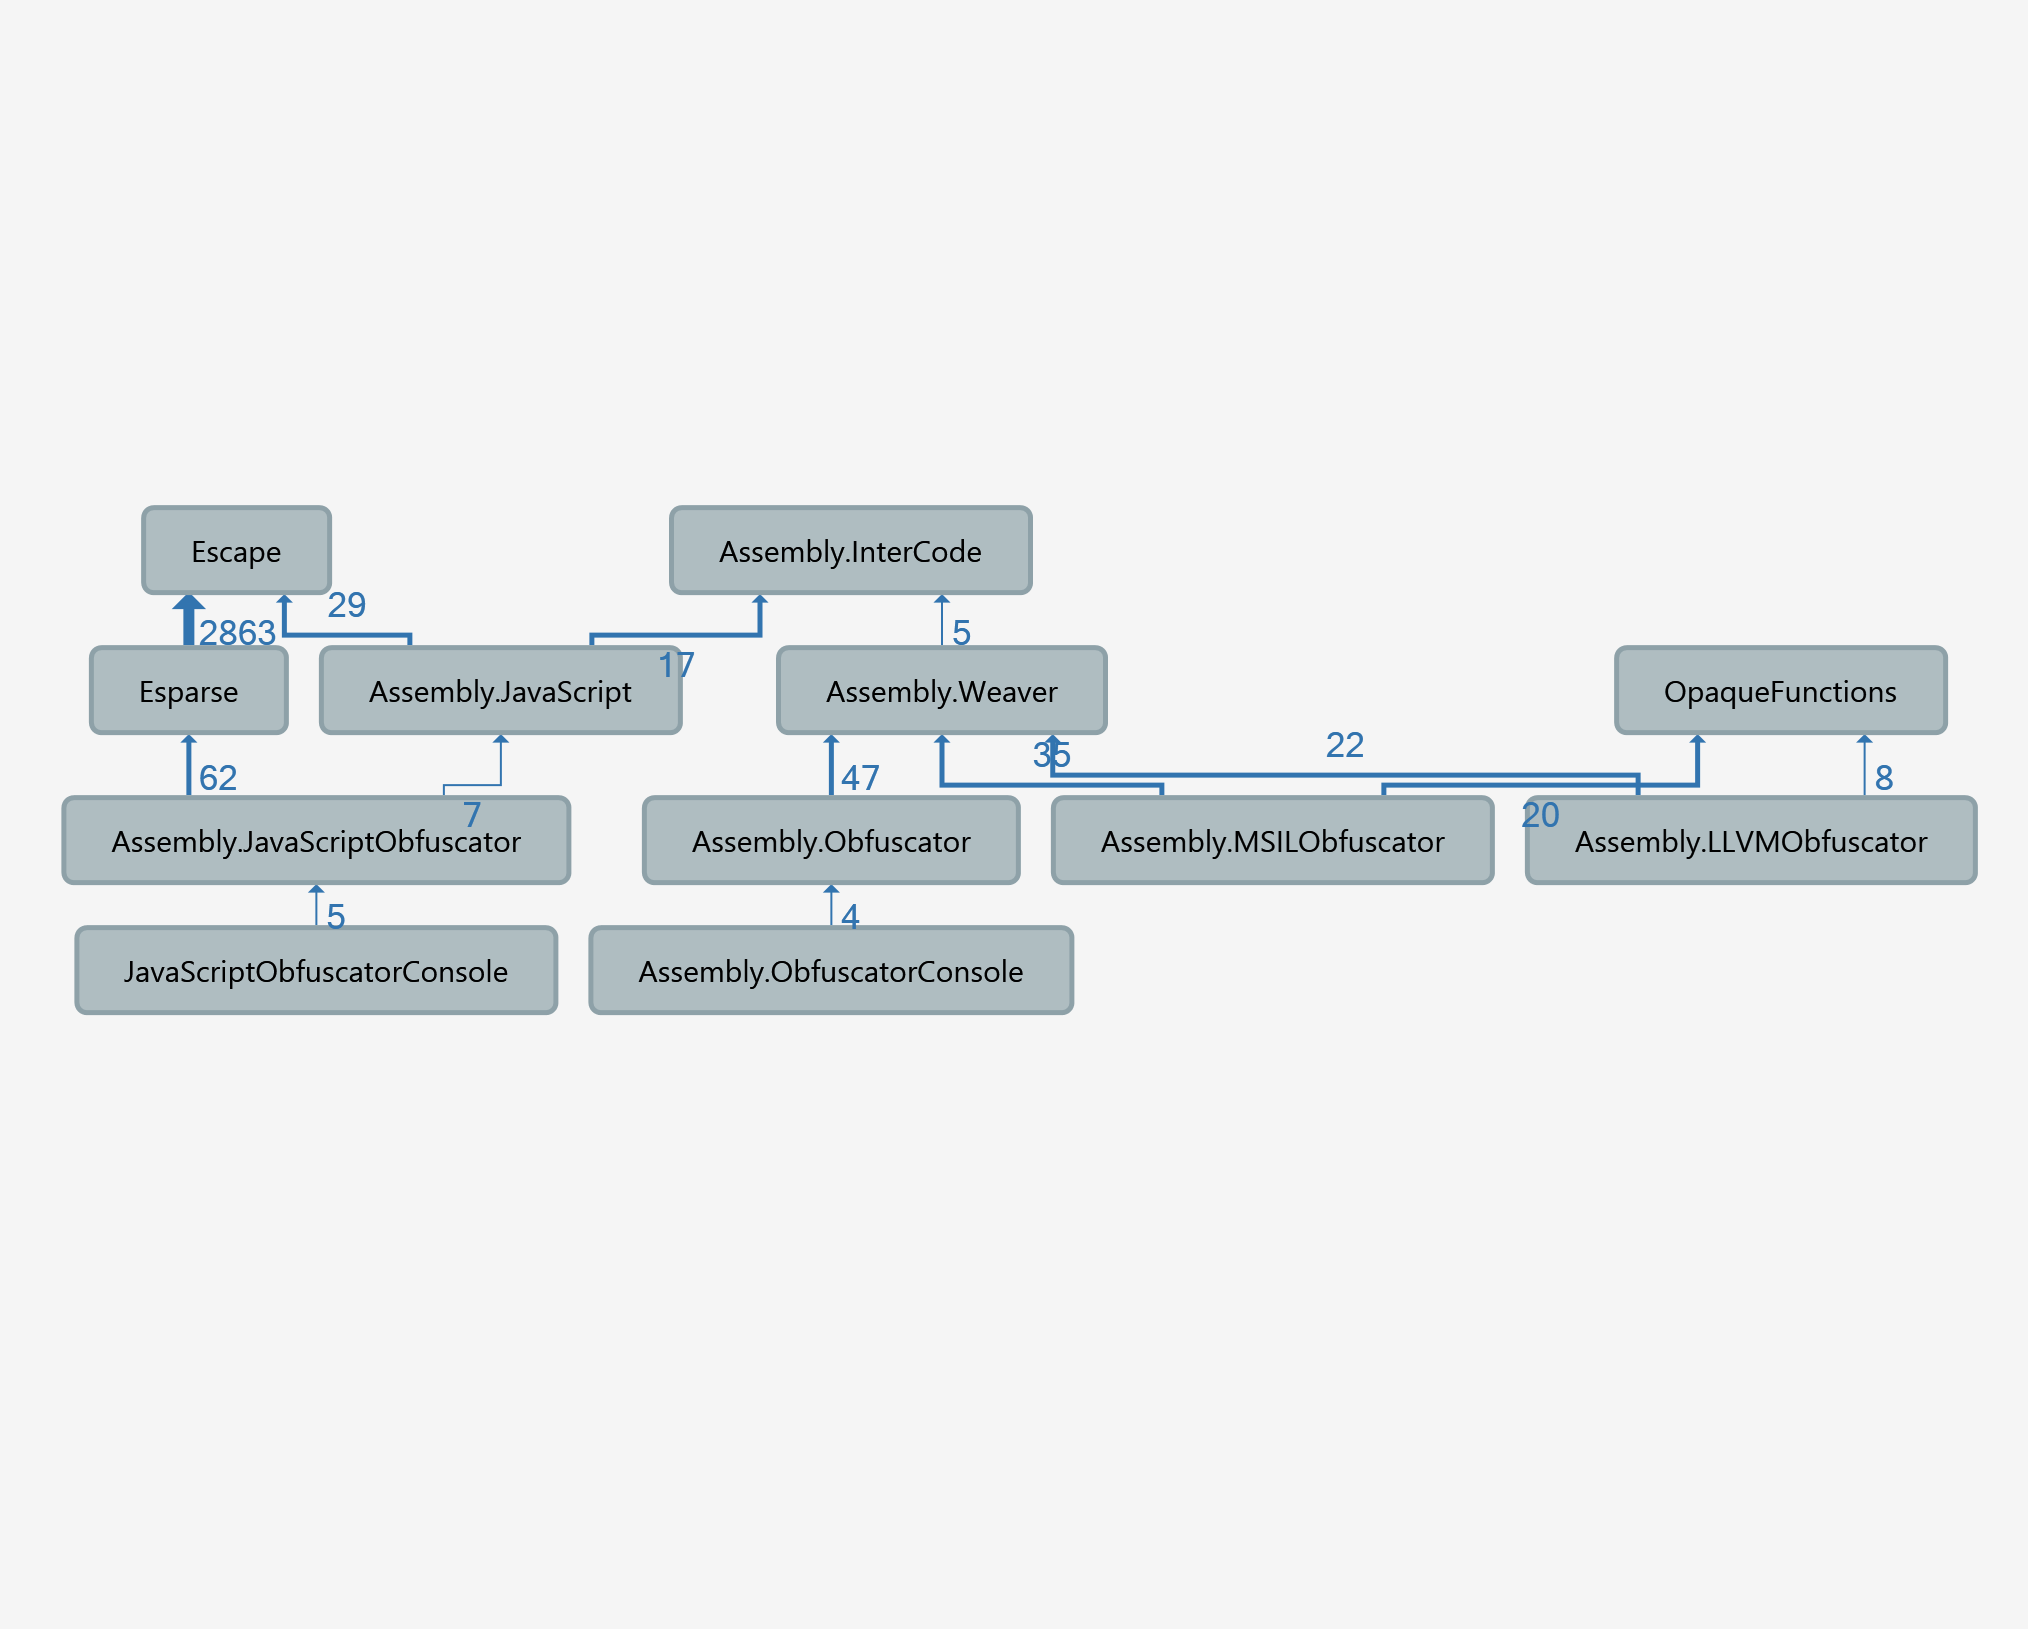
\includegraphics[width=1.0\linewidth]{DependenciesGraph.png}
\end{figure}
\end{frame}

\begin{frame}
\frametitle{Инструменты}
\begin{figure}[H]
  \center
  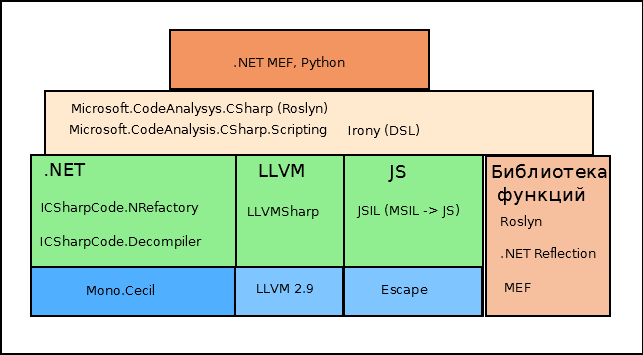
\includegraphics[width=1.0\linewidth]{Tools.png}
\end{figure}
\end{frame}


\begin{frame}
\frametitle{Общая схема}
\begin{itemize}
  \item Исходная программа обрабатывается в несколько проходов
  \item В каждом проходе программа разбивается на блоки операторов, например на простые блоки-вершины управляющего графа.
  \item Посещаются операторы каждого блока, проверяется применимость преобразований к ним.
  \item Для операторов, к которым применимы преобразования, они применяются.
  \item Записывается полученный байт-код или исходный код модифицированной программы.
\end{itemize}
\end{frame}

\begin{frame}
\frametitle{InterCode}
\begin{tcolorbox}[colback=green!5,colframe=green!40!black,title=пример]
SumTransform: a + b => a + 1 + b - 1 + c  \{ var c = FormIntOpaqueValue(0);\}
\end{tcolorbox}
здесь
\begin{itemize}
  \item SumTransform, DivTransform - имена преобразований
  \item выражение1 => выражение2 означает замену оператора (или его части) эквивалентного левой части на правую
  \item текст в скобках \{ \} задает значения новых переменных, в примере это вызов непрозрачной функции
\end{itemize}
\end{frame}


\begin{frame}
\frametitle{Применение правил}
\begin{figure}[H]
  \center
  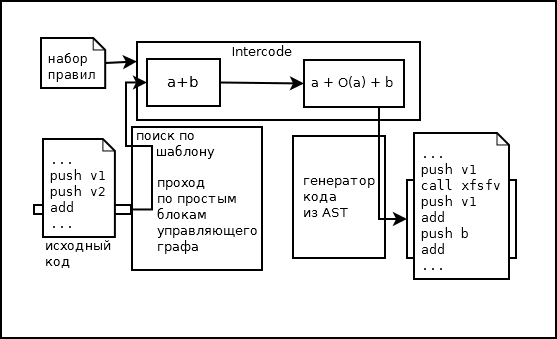
\includegraphics[width=1.0\linewidth]{RuleApplication.png}
\end{figure}
\end{frame}


\defverbatim[colored]\lstI{
\begin{lstlisting}[language=C++,basicstyle=\ttfamily,keywordstyle=\color{red}]
    o = PyAssembly.Manager(..., "LLVM")
    p = o.GetPass("all_cfg")
    o.AddParameter("useCodeGenerator", "true")
    o.AddParameter("constant1", "Opaque1LoopInt")
    p.CreateRule(name = "1", fromExpr = "a+b", 
    to = "a+b", action = " ")
    p.CreateRule(name = "2", fromExpr = "a-b", 
    to = "a-b+1-1", action = " ")
    p.CreateRule(name = "3", fromExpr = "a*b", 
    to = "a*b*c", 
    action = "var c=FormIntOpaqueValue(1); ")
    o.AddPass(cfgPass)
    o.Open(path); o.Run()
    o.Save(path)
\end{lstlisting}
}

\begin{frame}{Пример запуска}{python}
\lstI
\end{frame}

\begin{frame}[fragile]{Дополнительные условия в правилах}{python}
\begin{verbatim}
    c = System.Func[IAttributable, bool](
    lambda function: function.HasAttribute("ObfuscateThis"))
    extraConditions = List[System.Object]()
    extraConditions.Add(extraCondition)
    p.CreateRule("1", "a+b", "a+b+0", "", extraConditions)
    p.CreateRule("2", "a-b", "a-b+0", "", extraConditions)
    p.CreateRule("3", "a*b", "a*b+0", "", extraConditions)
    o.AddPass(cfgPass)
    
    Это применит замены только к функциям 
    с атрибутом [ObfuscateThis]
\end{verbatim}
\end{frame}



\begin{frame}
\frametitle{Типы}
\begin{tcolorbox}[colback=green!5,colframe=green!40!black,title=пример]
SumTransform: a + b => a + 1 + b - 1  \{ int a; int b;\}
\end{tcolorbox}
\begin{itemize}
  \item можно указать типы для всех участвующих переменных
  \item типы проверяются без неявных преобразований
  \item расширить проверки типов достаточно просто
\end{itemize}
\end{frame}

\begin{frame}[fragile]
\frametitle{Ветвления}
\begin{tcolorbox}[colback=green!5,colframe=green!40!black,title=пример]
\begin{verbatim}
1: _FunctionStart=>hub{var hub=AddControlHub();}
2: _Break=>entry{var entry=AddHubEntryAfter(current);}
3: _FunctionEnd=>nop{var nop=FinilizeHub();}
\end{verbatim}
\end{tcolorbox}
\begin{itemize}
  \item можно перенаправлять операторы ветвлений
  \item нужны проверки корректности
  \item не достаточно удобно добавлять правила
\end{itemize}
\end{frame}

\begin{frame}[fragile]{Пример MSIL}
правило: a-b => a - 24 - b + 24
\begin{columns}
 
\column{0.3\textwidth}

sub =>

\column{0.7\textwidth}
\begin{tcolorbox}[colback=green!5,colframe=green!40!black,title=результат]
\begin{verbatim}
stloc a_backup
ldloc a_backup
ldc.i4 24
sub
ldloc b_backup
sub
ldc.i4 24
add


\end{verbatim}
\end{tcolorbox}
\end{columns}
\end{frame}

\begin{frame}[fragile]{Пример вставки функций MSIL}
правило: a+b => a + 3 + b - 3 + f(), f = sin(pi/3) + sin(-pi/3)
\begin{columns}
 
\column{0.1\textwidth}

add =>

\column{0.9\textwidth}
\begin{tcolorbox}[colback=green!5,colframe=green!40!black,title=результат]
\begin{multicols*}{2}
\begin{verbatim}
stloc a_backup
ldloc a_backup
ldc.i4 3
add
ldloc b_backup
add
ldc.i4 3
sub
ldc.r8 1,0471975511966
call Double Sin(Double)
ldc.r8 -1,0471975511966
call Double Sin(Double)
add
stloc V_22
ldloc V_22
add
\end{verbatim}
\end{multicols*}
\end{tcolorbox}
\end{columns}
\end{frame}

\begin{frame}[fragile]{Пример LLVM}
правило: a * b => a * b * 3 / 3
\begin{columns}
 
\column{0.2\textwidth}

\%tmp2 = mul i32 \%1, \%tmp1

\column{0.8\textwidth}
\begin{tcolorbox}[colback=green!5,colframe=green!40!black,title=результат]
\begin{verbatim}
%tmp0012 = alloca i32
  store i32 3, i32* %tmp0012
  %tmp0023 = load i32, i32* %tmp0012
  %tmp0034 = mul i32 %tmp0023, %tmp0001
  %tmp0045 = alloca i32
  tore i32 3, i32* %tmp0045
  %tmp0056 = load i32, i32* %tmp0045
  %tmp0067 = sdiv i32 %tmp0056, %tmp0034
\end{verbatim}
\end{tcolorbox}
\end{columns}
\end{frame}

\begin{frame}[fragile]{Пример вставки функций LLVM}
правило: a * b => a * b * c, c = Opaque1LoopInt()
\begin{columns}
     
\column{0.2\textwidth}

\%tmp2 = mul i32 \%1, \%tmp1

\column{0.8\textwidth}
\begin{tcolorbox}[colback=green!5,colframe=green!40!black,title=результат]
\begin{verbatim}
  %tmp1 = mul i32 %tmp1, %1
  %tmp2 = call i32 @Opaque1LoopInt()
  %tmp3 = mul i32 %tmp2, %tmp1
  %tmp4 = mul i32 %1, %tmp0
  ...
  define i32 @Opaque1LoopInt() {
  "3":
  %loc0 = alloca double
  ...
  "4": ...
  
\end{verbatim}
\end{tcolorbox}
\end{columns}
\end{frame}

\begin{frame}[fragile]{Пример JavaScript}
\begin{tcolorbox}[colback=blue!5,colframe=green!40!black,title=вход]
\begin{verbatim}
var res1 = (a - b) | 0; // result = 3
var res2 = (a * b) | 0; // result = 18
var res3 = (a / b) | 0; // result = 2
var res4 = (((a + b) | 0) - 1) | 0;
\end{verbatim}
\end{tcolorbox}

\begin{tcolorbox}[colback=green!5,colframe=green!40!black,title=результат]
\begin{verbatim}
var res0 = ((((a + 2) + b) - 2)) | 0; 
var res1 = ((((a - 42) - b) + 42)) | 0;
var res2 = ((((a * b) * 2) / 2)) | 0; 
var res3 = (((a * 1) / b)) | 0; // result = 2
var res4 = ((((((a + 3) + b) - 3)) | 0) - 1) | 0; 
\end{verbatim}
\end{tcolorbox}
\end{frame}

%\usebackgroundtemplate{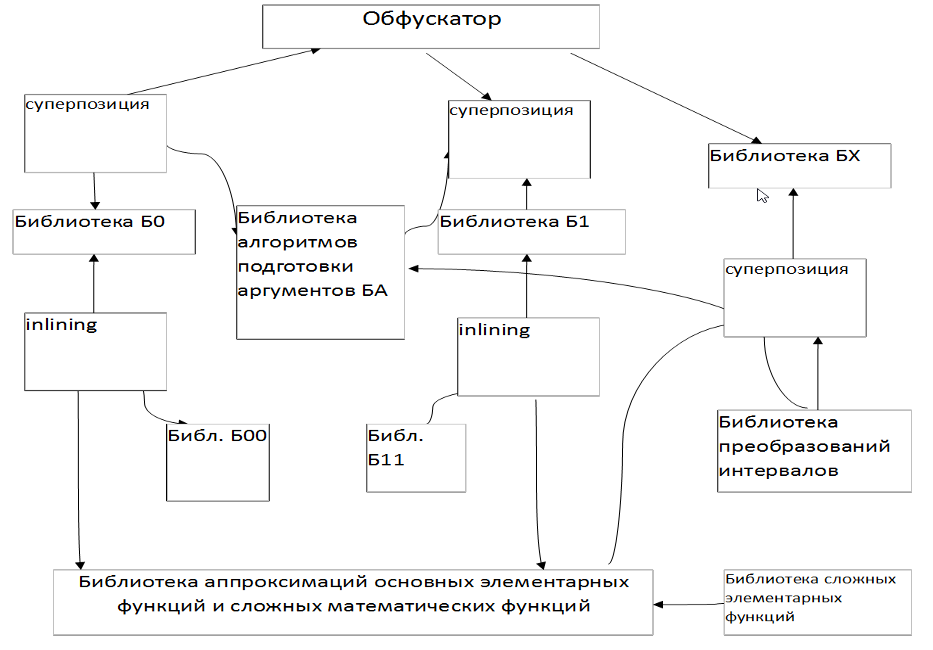
\includegraphics[width=\paperwidth,height=0.9\paperheight]{FunctionLibrary.png}}%
\begin{frame}
\frametitle{Структура библиотеки непрозрачных функций}
\begin{figure}[H]
  \center
  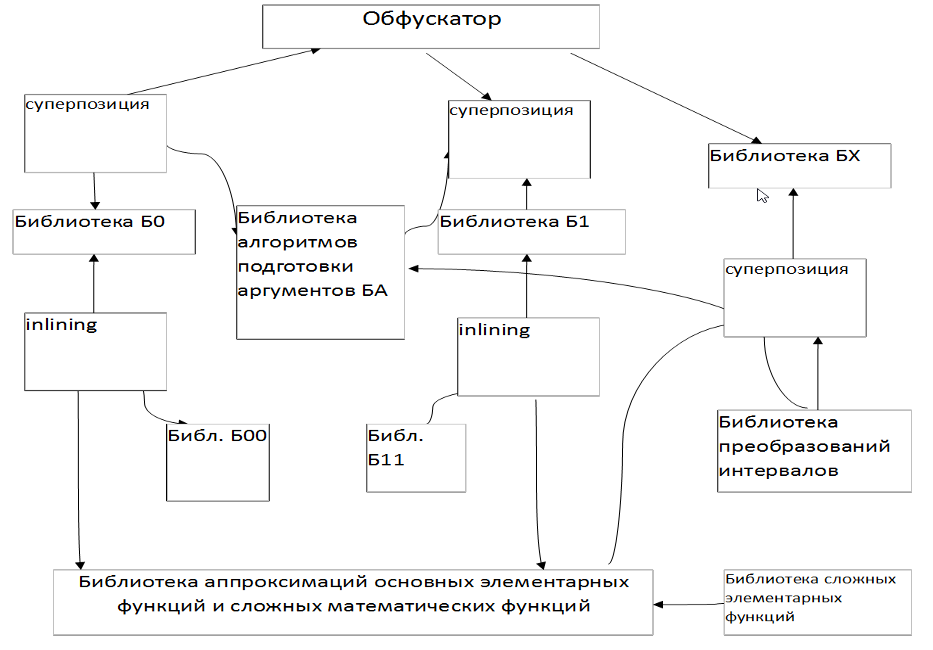
\includegraphics[width=1.0\linewidth, height=0.9\paperheight]{FunctionLibrary.png}
\end{figure}
\end{frame}

%\usebackgroundtemplate{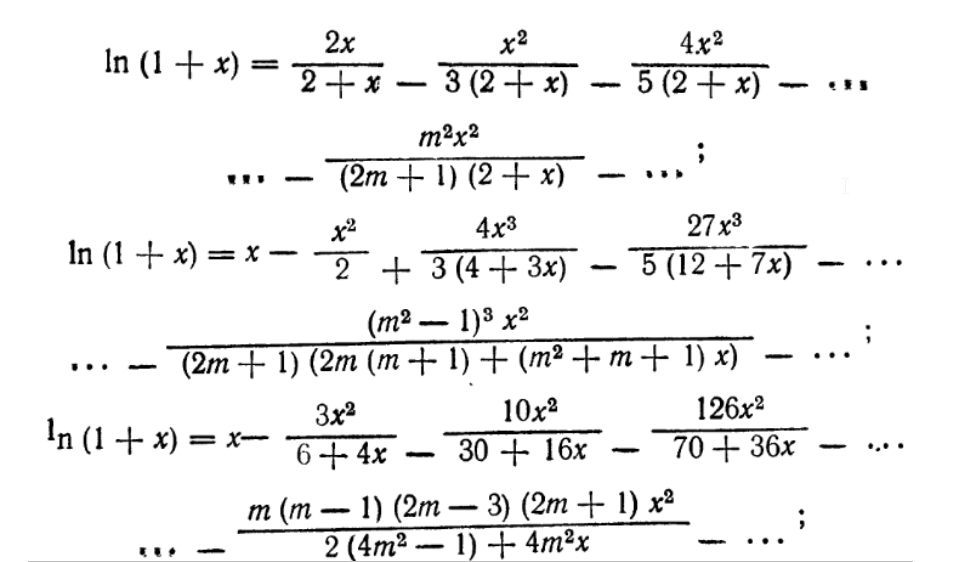
\includegraphics[width=\paperwidth,height=0.9\paperheight]{Formulae.png}}%
\begin{frame}
\frametitle{Пример простой функции}
\begin{figure}[H]
  \center
  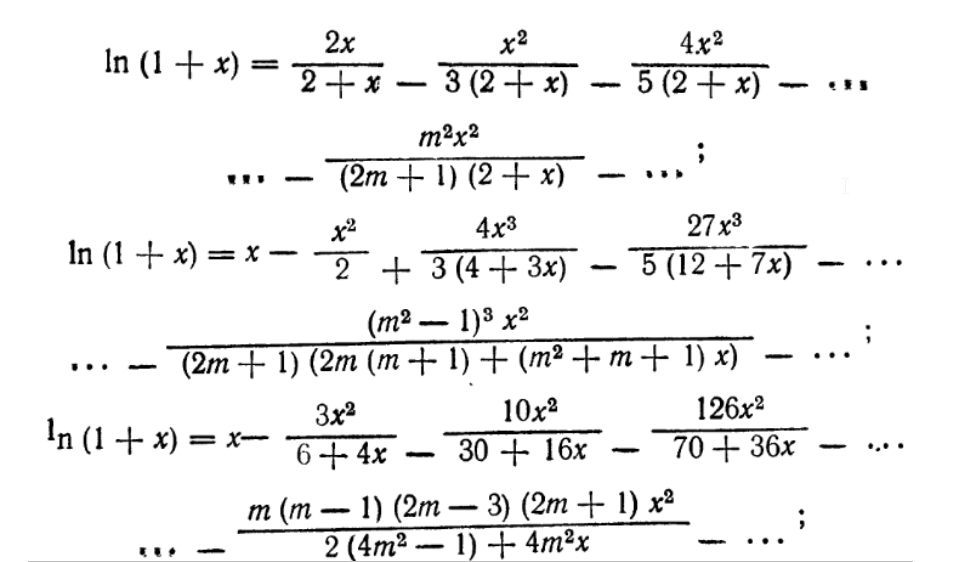
\includegraphics[width=1.0\linewidth]{Formulae.png}
\end{figure}
\end{frame}

\usebackgroundtemplate{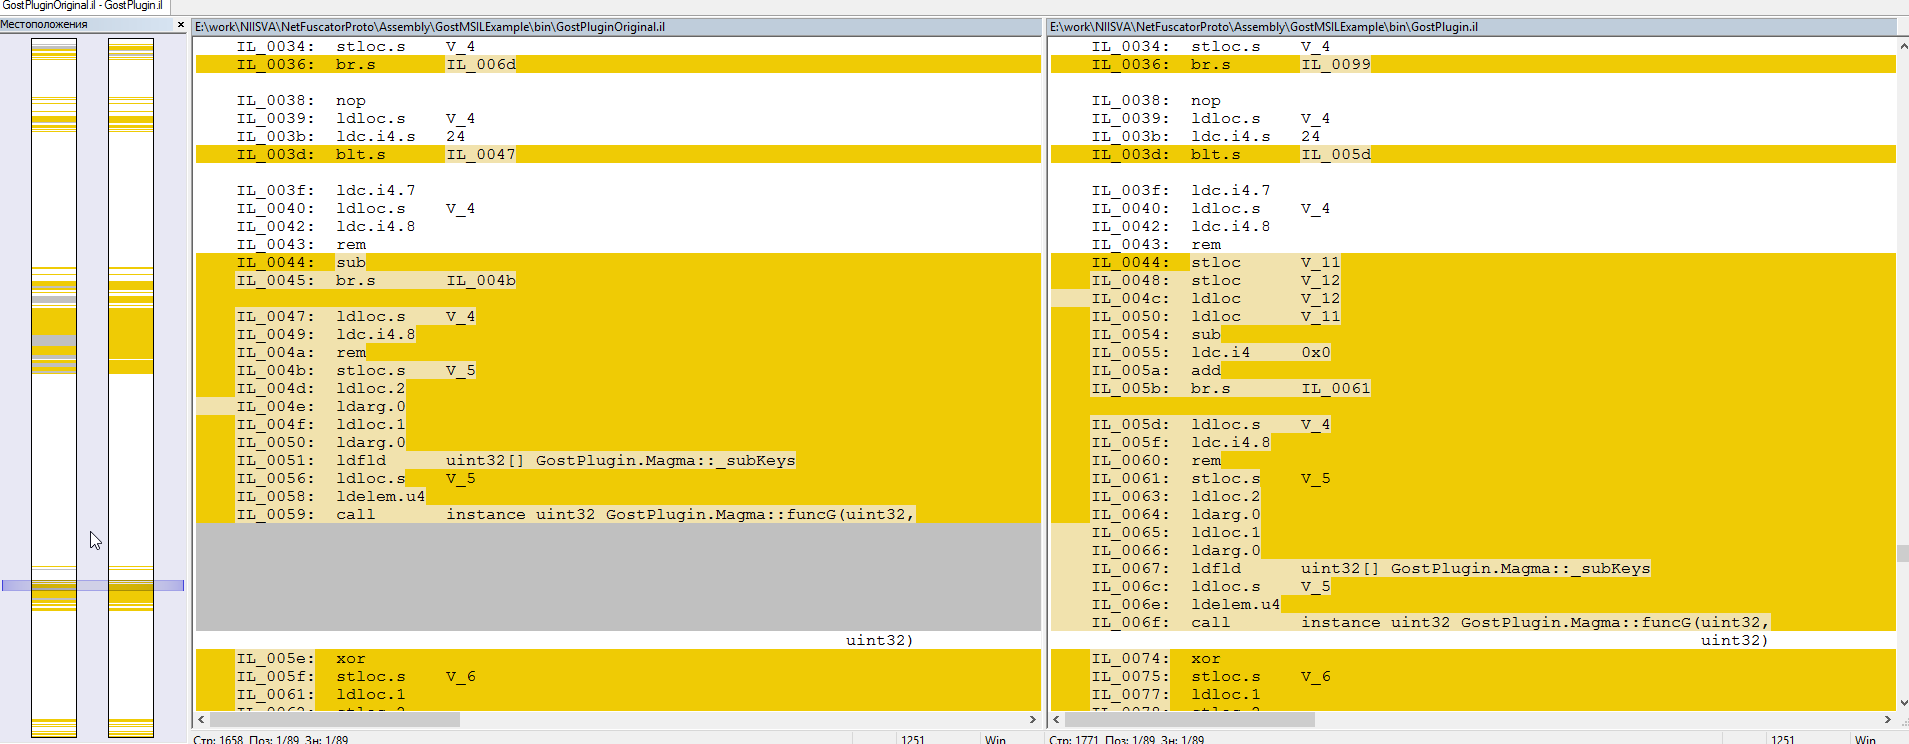
\includegraphics[width=\paperwidth,height=0.9\paperheight]{MSILDiffExample.png}}%
\begin{frame}
\frametitle{Рабочий пример MSIL - ГОСТ Р 34.12-2015. }
\textbf{сделано замен: 39,
всего инструкций: 1233}
%\begin{figure}[H]
  %\center
  %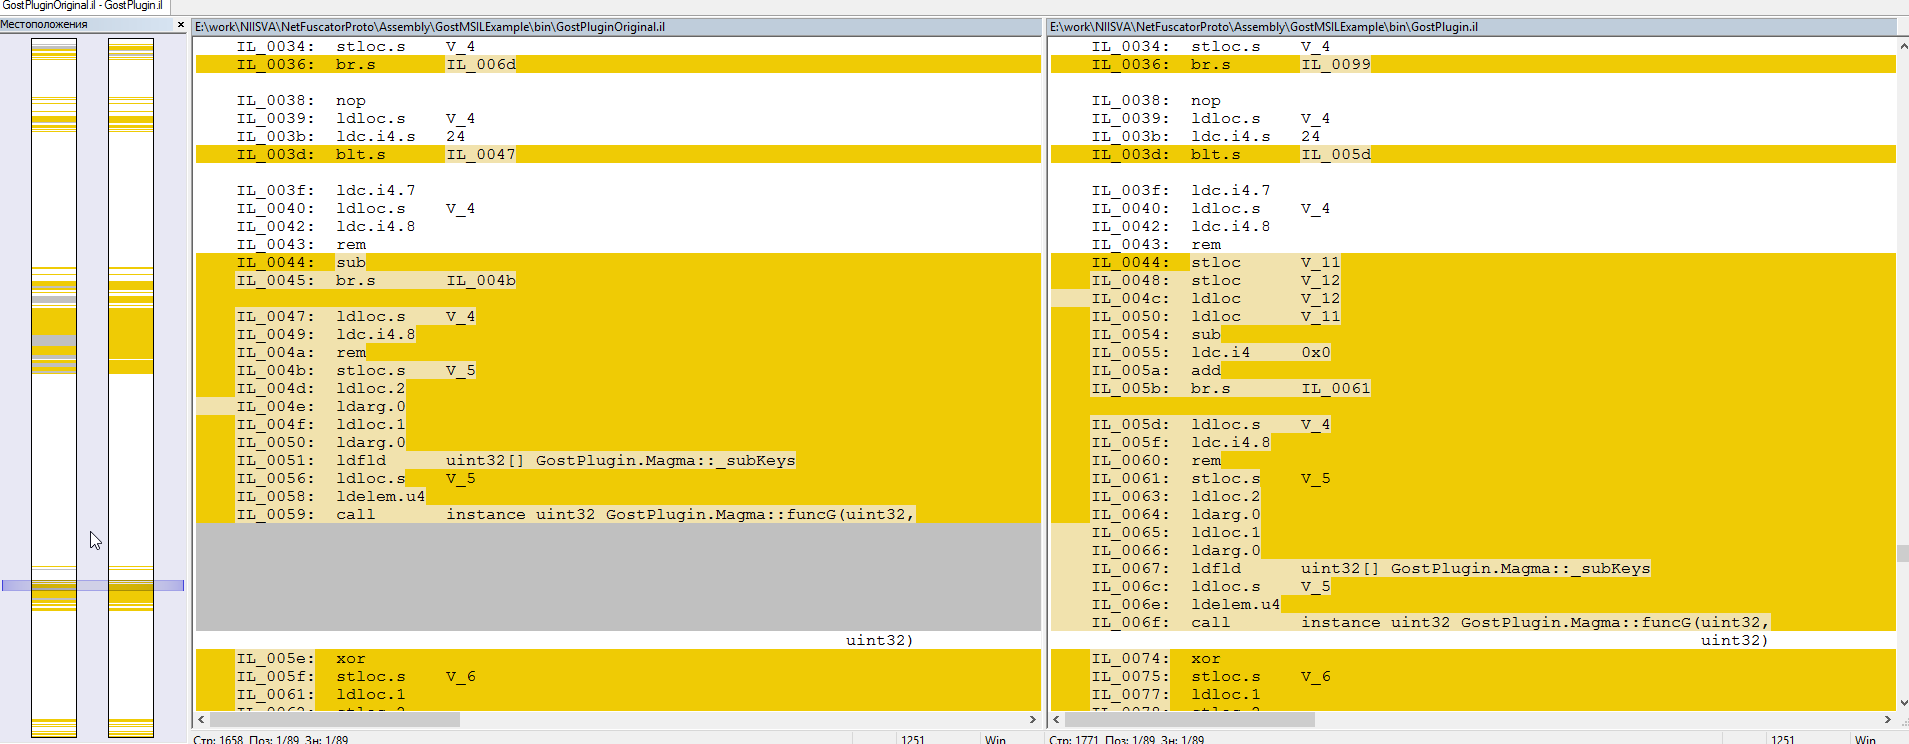
\includegraphics[width=1.0\linewidth]{MSILDiffExample.png}
%\end{figure}
\end{frame}

\usebackgroundtemplate{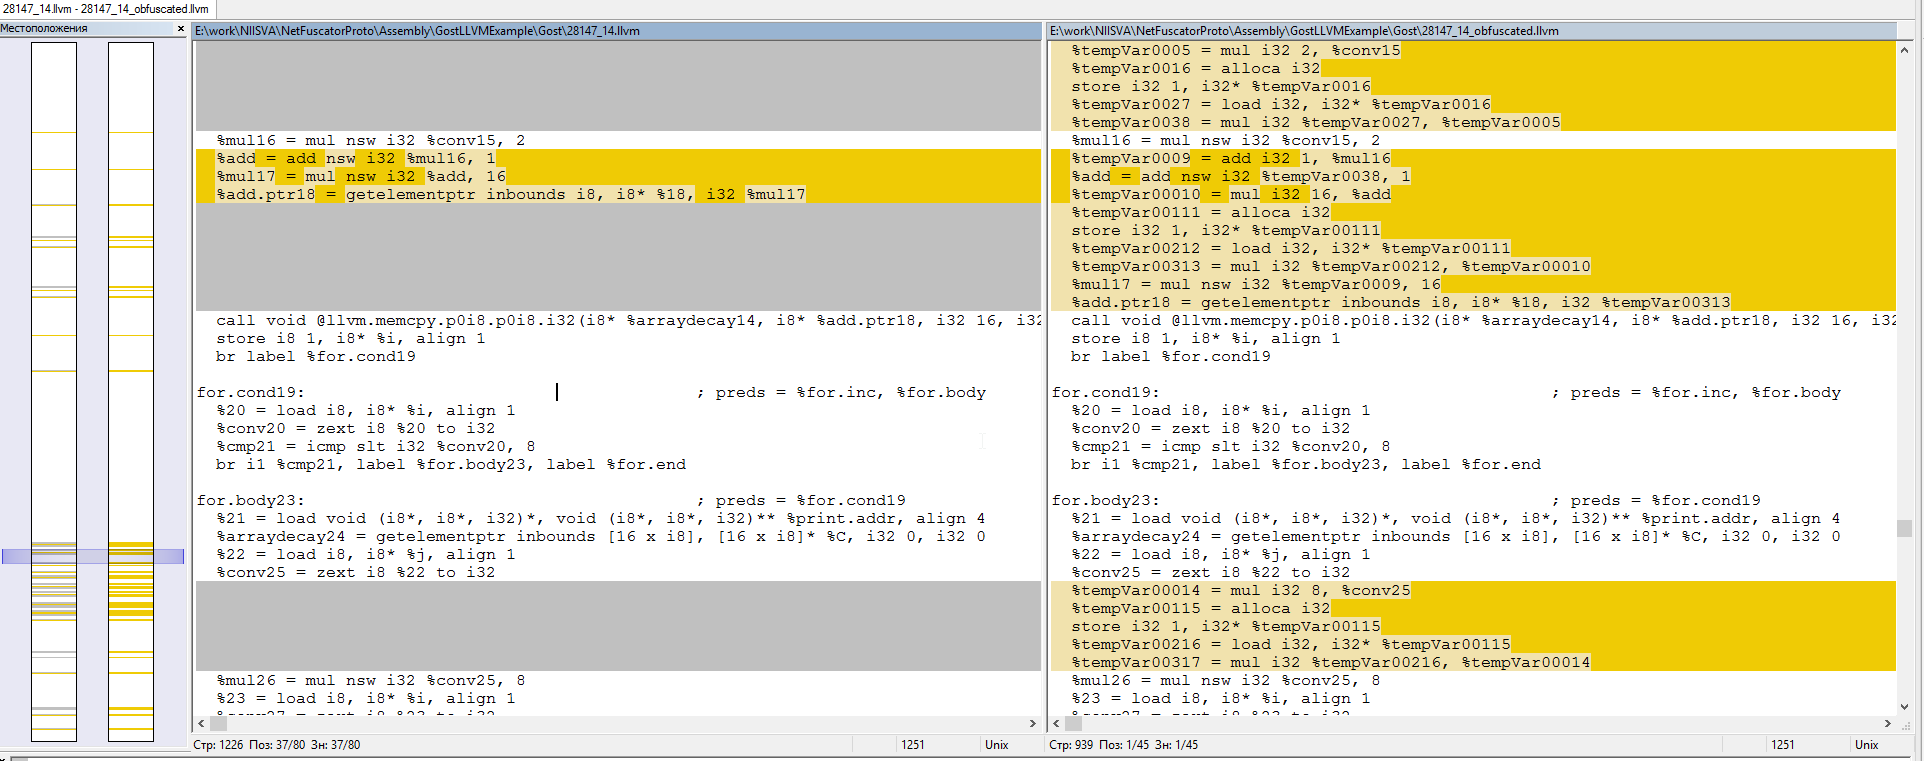
\includegraphics[width=\paperwidth,height=0.9\paperheight]{LLVMDiffExample.png}}%
\begin{frame}
\frametitle{Рабочий пример LLVM - ГОСТ Р 34.12-2015. }
\textbf{сделано замен: 98,
всего инструкций: 5103}
%\begin{figure}[H]
%  \center
%  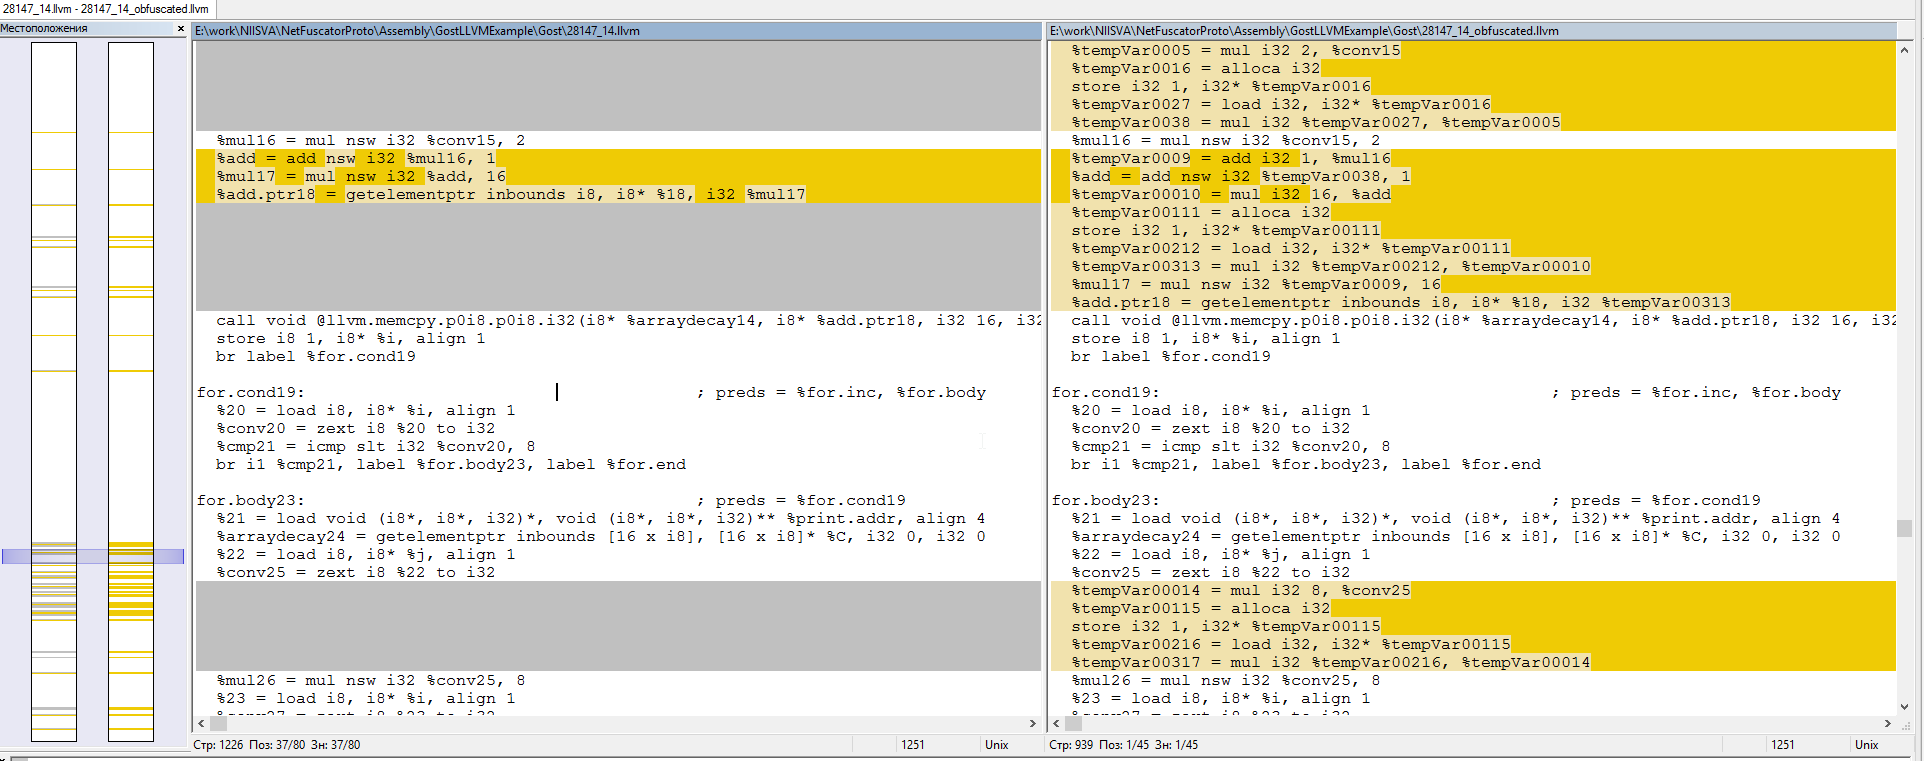
\includegraphics[width=1.0\linewidth]{LLVMDiffExample.png}
%
%\end{figure}
\end{frame}

\usebackgroundtemplate{}%
\begin{frame}
\frametitle{Другие примеры и большие сборки. }
\begin{enumerate}
  \item Linpack и Whetstone для .NET (сборка 20-30кб)
     сделано замен: 252,
     всего инструкций: 2628,
     время работы около минуты 
  \item MathNet.Numerics (сборка 1.5мб)
     время работы больше часа, потребляет больше 10Гб памяти...
\end{enumerate}
\end{frame}

\begin{frame}
\frametitle{Нерешенные проблемы}
\begin{enumerate}
    \item обход управляющего графа в JavaScript и использование общего интерфейса
    \item вывод типов в JavaScript - сложная задача в общем случае
    \item оптимизация времени работы обфускатора MSIL (использование "тяжелых" инструментов)
    \item неоптимальная организация обфускатора LLVM из-за использования С-интерфейсов
    \item как не замедлить программу модификациями? Пример для ГОСТ c MSIL может легко замедлить его в 5-10 раз из-за вставки кода во вложенные циклы.
    \item разработка эквивалентных преобразований
\end{enumerate}
\end{frame}
    

\begin{frame}
\frametitle{Сценарии развития}
\begin{enumerate}
    \item семейство обфускаторов, объединенных общим подходом (описанием преобразований, алгоритмом их выбора)
    \begin{enumerate}
        \item улучшенная работа с динамическими языками за счет использования уже имеющихся инструментов
        \item сложнее обеспечить какой-то общий способ модификации потока управления 
    \end{enumerate}
    \item  многоязыковая среда с обработкой нескольких языков через обобщенный метаязык - сильнее ограничивает работу с каждым из языков и сложнее в реализации
    
\end{enumerate}
\end{frame}

\end{document} 